\documentclass[a4paper,oneside,11pt]{article}
\usepackage{graphicx}
\usepackage{ tipa }
\usepackage{hyperref}
\usepackage{titling}
\usepackage{blindtext}
\usepackage{enumitem}
\usepackage{eurosym}
\title{RASD}
\author{Daniele Montesi, Nicola Fossati, Francesco Sgherzi}
\date{\today}
\begin{document}
    \begin{titlingpage} 
        \begin{center}
            
\includegraphics[height=5cm]{assets/Logo_Politecnico_Milano.png}\\
            \vspace{4cm}
            \begin{huge} 
                \textbf{\thetitle} \\
            \end{huge}
            \vspace{0.3cm}
            \begin{Large}
                \textit{Software Engineering 2 Project - TrackMe} \\
            \end{Large}
        \end{center}
        \begin{large}
            \vspace{4cm}
            \textbf{Authors}
            \begin{itemize}
                \item Daniele Montesi - \textit{912980} 
                \item Nicola Fossati - \textit{915244}
                \item Francesco Sgherzi - \textit{915377}
            \end{itemize}
        \end{large}
    \end{titlingpage}
    \newpage
    \tableofcontents
    \newpage
    \section{Introduction}
    
        \subsection{Purpose}
            The main purpose of this document is to exhaustively describe the Data4Help main architecture, its parts and how they interact. There is also a chapter that covers the user interface.

The main recipients of this document are the project manager, developers and testers, but it can also be useful for further development reference and maintenance.
        \subsection{Scope}
            % To define the scope of the product we can use ``The World \& Machine'' approach by M. Jackson and P. Zave.
% We can define the real world entities that interact with the system (the World), the entities that belong to the system (the Machine) and the shared phenomena (the intersection of the two other sets).

% TODO: add image here

The \textit{The World and the Machine} approach is used in defining the scope of the project.
By defining the real world entities that interact with the system and the properties of the system itself we can determine the intersection between the two sets: the \textit{shared phenomena}.
\begin{center}
    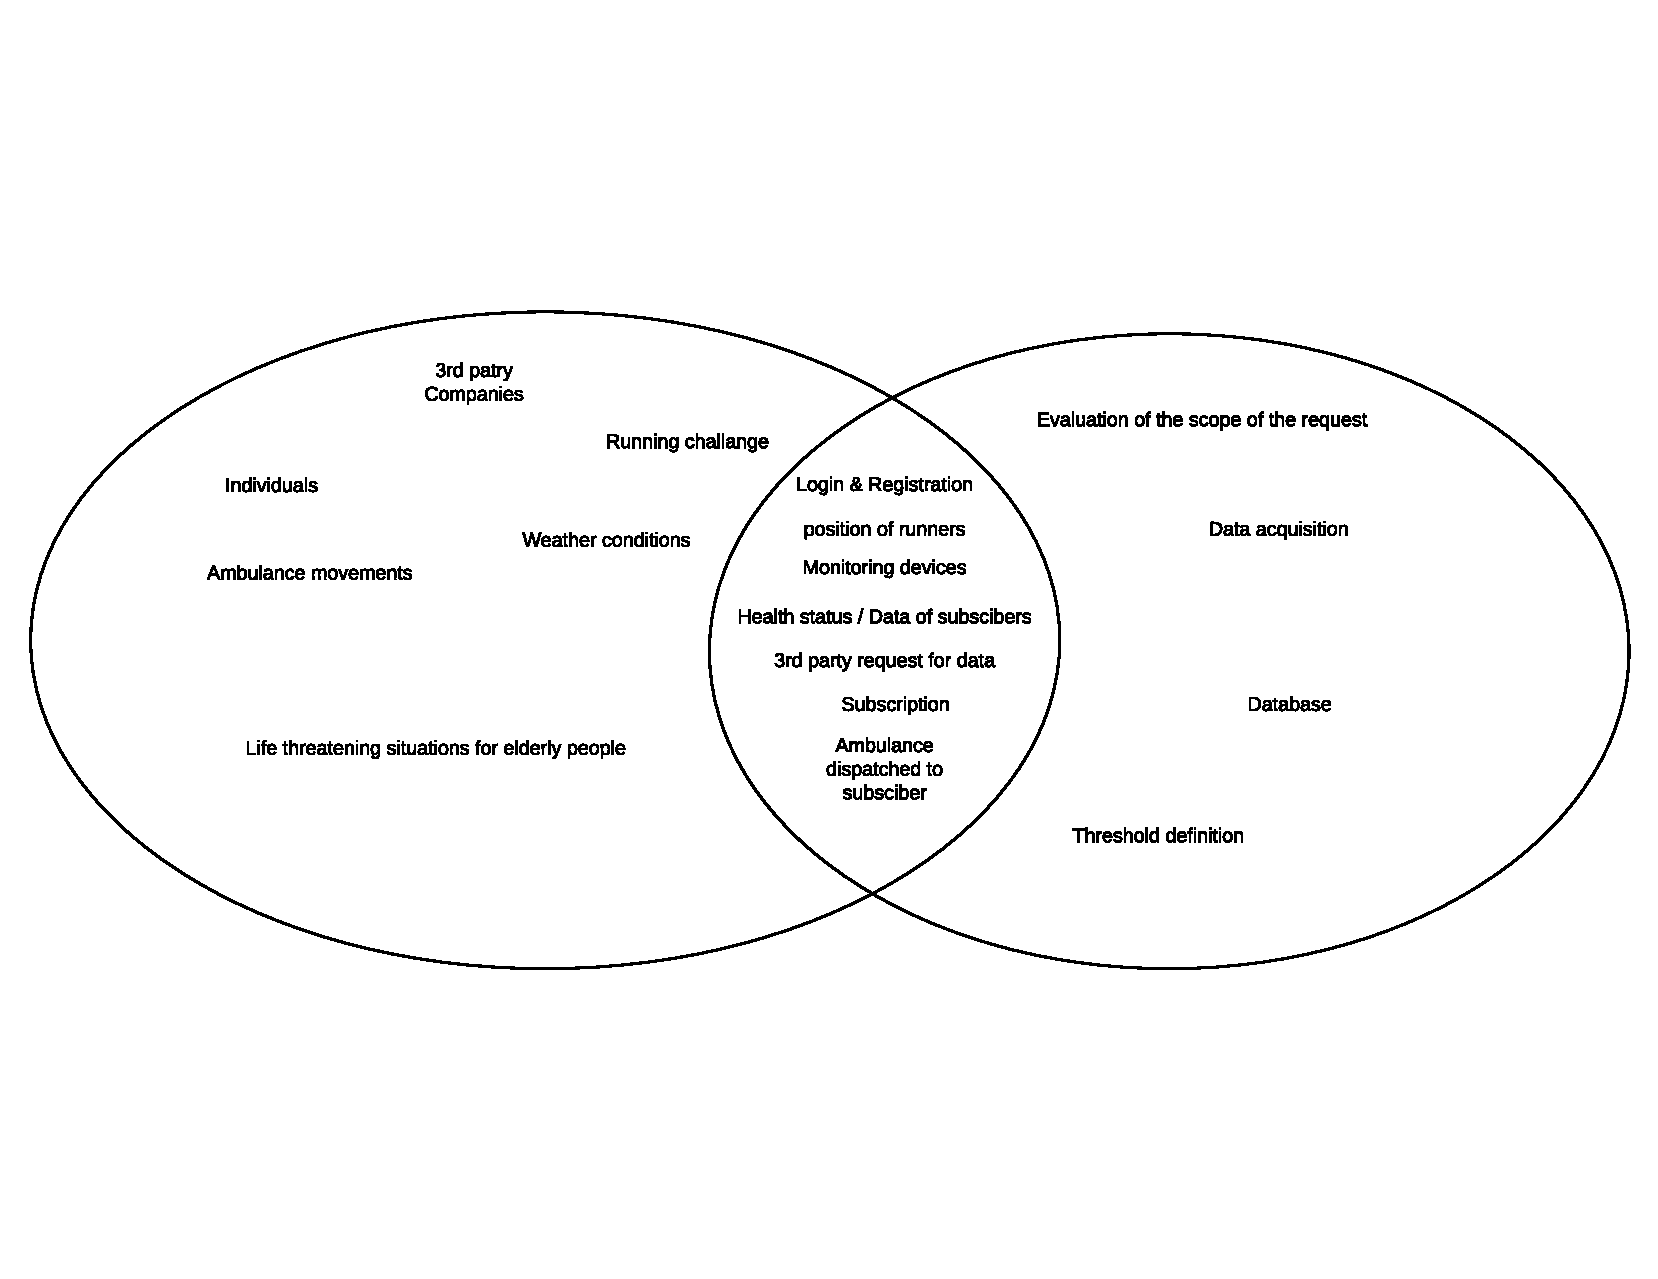
\includegraphics[height=8cm,keepaspectratio]{assets/twatm.pdf}
\end{center}

The system-to-be uses 3 components with different roles in order to work:
\begin{itemize}
    \item \textbf{Data4Help SmartWatch App}: Acquires the data from the smartwatch sensors (heart rate, sleep quality, position, phisical activities) and sends them via Bluetooth to the Data4Help Mobile App
    \item \textbf{Data4Help Mobile App}: Gathers data from the smartwatch, shows various statistics, and sends them to the Data4Help Core Database. Each user can choose which service subscribe to
    \item \textbf{Data4Help Website}: Gives third-party companies the ability to request data, either anonymized or user specific. Moreover, it allows run organizers to define the path of the run and the spectators to see the position of all runners on a map.
    \item \textbf{Data4Help Core}: is intended to connects all other components together providing the logic of the application. It is also responsible for the acceptance of all third-parties requests of data. It also evaluate health status of individuals deciding whether is at risk or not.
\end{itemize}

The list below shows the main goals the system should be able to accomplish:

\begin{itemize}
    \item \textbf{G1}: The system should be able to read sensor data from smart devices.
    \item \textbf{G2}: The system should be able to show acquired data via the Mobile App and the Website.
    \item \textbf{G3}: The system should allow users to register.
    \item \textbf{G4}: The system should allow companies to register.
    \item \textbf{G5}: The system should allow registered companies to request data either from specific individuals or from an anonymized group of individuals.
    \item \textbf{G6}: The system should allow users to accept or decline a company request for their specific data.
    \item \textbf{G7}: The system should provide a payment method to registered companies requesting user data. %eviterei di specificare payment system
    \item \textbf{G8}: The system should be able to communicate directly to ambulances.
    \item \textbf{G9}: The system should be able to react to the lowering of the health parameters below threshold in less than 5 seconds and send the position of the person to the ambulance system. 
    % \item \textbf{G10}: The system should should allow organizers to define the path for the run.
    \item \textbf{G10}: The system should be able to communicate interoperably with its services: \textit{AutomatedSOS} and \textit{Track4Run}
    \item \textbf{G11} The system should allow run organizers to register.
    \item \textbf{G12} If a run organizer is registered, it can define a run i.e. it can define the path that the participants should follow.
    \item \textbf{G13} A user should be able to enroll to a run.
    \item \textbf{G14} Spectators of a run should be able to see each participant's position on a map.
\end{itemize}

%A health data aggregator app that gives the user the ability to monitor all 

%is intended to offer all the functionalities of the service to the individuals, including heart rate monitoring, sleep monitoring




        \subsection{Definitions, Acronyms, Abbreviations}
            \renewcommand{\arraystretch}{1.5}
\begin{center}
    \begin{tabular}{|l|r|}
        \hline
        \textbf{i.e.} & \textit{Id est}, that is  \\
        \hline
        \textbf{w.r.t} & with respect to  \\
        \hline
        \textbf{w.l.o.g.} & without loss of generality \\
        \hline
        \textbf{The company} & TrackMe \\
        \hline
        \textbf{BLE} & Bluetooth Low Energy \\
        \hline
    \end{tabular}
\end{center}
        \subsection{Revision history}
        \subsection{Reference documents}
            \begin{itemize}
\item \textbf{|REFD1|} \href{https://en.wikipedia.org/wiki/Model–view–presenter}{\textbf{MVP}}

\item \textbf{|REFD2|} \href{https://standards.ieee.org/standard/1016-2009.html}{\textbf{IEEE Std 1016-2009 Standard for Information Technology, Systems Design, Software Design Descriptions}}

\item \textbf{|REFD3|} \href{https://it.wikipedia.org/wiki/Representational_State_Transfer}{\textbf{Representational State Transfers}}

\end{itemize}
        \subsection{Document structure}
        This document is divided in the following chapters:
\begin{description}
\item[Implemented requirements] Explains which functional requirements outlined in the RASD are accomplished, and how they are performed.
\item[Design choices] provides reasons about the implementation decisions taken in order to develop the application.
\item[Source code structure] explains and motivates how the source code is structured both in the front end and in the back end.
\item[Testing] provides the main testing cases applied to the the application
\item[REST API] describes the API implemented for the application.
\end{description}
        
    \newpage
    \section{Overall description}
        \subsection{Product perspective}
            Data4Help Core is the central component of the system that connects all the other parts of the structure.
\begin{center}
    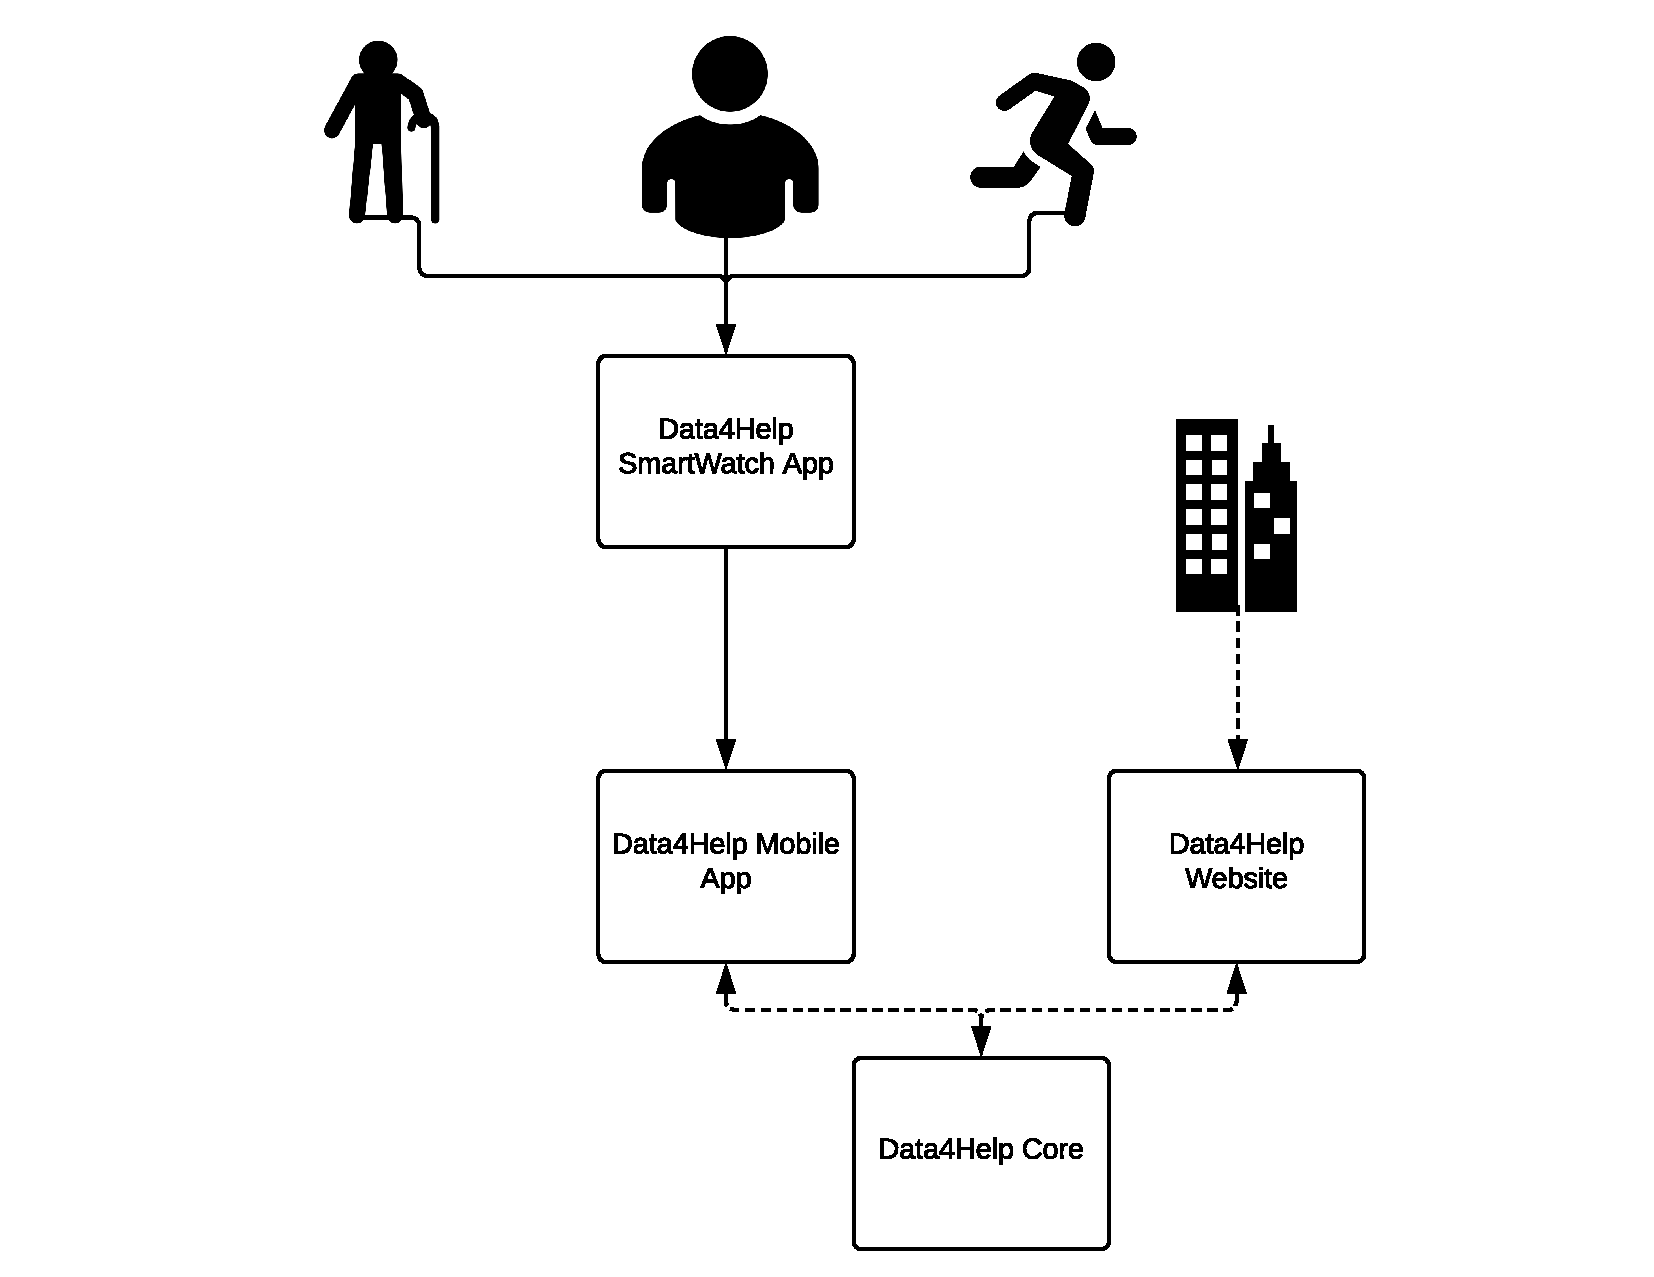
\includegraphics[height=7cm]{assets/useflow.pdf}
\end{center}

The Smartwatch App should be directly connected to the Mobile App to acquire data and let them be shown in the smartphone. In turn, the Mobile App has to communicate with the Data4Help Core that will register the data of the user. The Data4Help Website should communicate with the Data4Help Core as well in order to query directly on the company database.
\newline
\textbf{
TODO: 
A. Product perspective: here we include further details on the shared phenomena and a
domain model (\textbf{class diagrams and statecharts)}
}
            \subsubsection{User Interfaces}
                \textbf{Data4Help Mobile App:}

The Mobile app should offer an easy interface aiming a user friendly experience of the customers. If should be possible to open a menu to navigate through the sub-sections. All the main functions (i.e. see history of activities, see account information) should be easy to access from any sub-section of the app. 
Descriptions of the pages has to be brief and concise.
To see the details of the statistics there should be an info button that shows detailed description about the related data.
If subscribed to the AutomatedSOS service, there should be a page showing the active controls on the user.
In case of using the Track4Run service, there is also the possibility to see the map of a programmed run and seeing on the map all the participants, and their positions. More detailed info of the runners can be shown by tapping on their icon on the map.

The application must follow a proper design for every different mobile operating system:
\begin{itemize}
    \item Android - \vspace{0.3cm} Material Design
    \item iOS - \vspace{0.3cm} ModernUI
\end{itemize}
The application should support all the screen resolutions available and optimize the item placement on the screen in the same way for every compatible device.
\newline
The user can configure the graphic of the widget visible from the Smartwatch only using the Mobile App component.



\textbf{Data4Help SmartWatch App} :
The Smartwatch app should provide \textbf{widgets} that let the customer see their daily activity.
There should be one widget for every type of data acquired by the device:
\begin{itemize}
    \item Sleep monitoring 
    \item Heart rate (if available)
    \item Pressure (if available)
\end{itemize}
The user can receive notifications about his activities in the Smartwatch and delete them through it.
\newline

\textbf{Data4Help WebSite}: The Website should offer an easy interface aiming a user friendly experience for the subscribed companies. The main menu should be visible on the top of the page, and must be used to navigate through the sub-sections. All the main functions (i.e. acquired data, account information, etc) should be accessible from any sub-section of the web page. 
Descriptions of the pages have to be clear and exhaustive.
\newline

\textbf{Data4Help Core:} This component does not have a user interface since it is intended to be accessible only by the qualified staff that manages it. 
            \subsubsection{Hardware Interfaces}
                \textbf{Data4Help Mobile App:} The application should require the location services in order to work. If GPS is unavailable on the mobile phone, it can be requested to the Smartwatch app and viceversa. If both unavailable, the application wouldn't work and show an error window to notify the user.
The app should also require a connection from either mobile network or Wi-Fi, but is sufficient to turn it at least once per day. If not, the app will notify the user asking to turn on connectivity. 

\textbf{Data4Help SmartWatch App:} As written for Data4Help Mobile app, but also requires bluetooth connectivity during the activities. If not available, an error message will appear on the Mobile app.

\textbf{Data4Help WebSite:} There is not any hardware interface needed for the WebSite component.

\textbf{Data4Help Core:} There is not any hardware interface needed for the Core component.
            \subsubsection{Software Interfaces}
                \begin{itemize}
    \item \textbf{Data4Help SmartWatch App}: Development will focus on the production of a WatchOS and a WearOS app in order to properly communicate with their respective smartphone app.\newline As an app built for the latest version of those OSes is also backwords compatible with their previous versions, there are no particular \textit{minimum version} requirements.
    By developing an app for WatchOS and WearOS, the app will reach the 84\% of all available Smartwatches.
    
    %%TODO: ADD LINK TO https://www.statista.com/statistics/466563/share-of-smart-wristwear-shipments-by-operating-system-worldwide/
    
    \item \textbf{Data4Help Mobile App}: Due to the fact that iOS and Android are the only OSes that provide a seamless integration with their smartwatch counterparts, the app will be developed for those platforms only.
    In order to support smartwatch communication there is a minimum version required for those OSes, namely:
    \begin{itemize}
        \item Android \textgreater \vspace{0.1cm} 4.4 (API level 19) (about 94,7\% of devices)
        %TODO: ADD REF TO https://data.apteligent.com/android/
        \item iOS \textgreater \vspace{0.4cm} 9.3 (about 96,3\% of devices)
        %TODO: ADD REF TO https://data.apteligent.com/ios/
    \end{itemize}
    
    \item \textbf{Data4Help Website}: It will require the use of a modern Web Browser to be accessed. It will work either on desktop and mobile Web Browsers.
    
    \item \textbf{Data4Help Core}: As the \textit{Core} component will need only to provide \textbf{REST} endpoints for the communication (with ambulance, Website, App) there are no specific requirements on this component.
\end{itemize}

% Add refd https://wearos.google.com/
            \subsubsection{Communication Interfaces}
                
In the system there are 2 types of communication.
\begin{enumerate}
    \item The Mobile App and the Web Site need a bidirectional channel with the Core component of the system to operate properly. \\
    This can be achived by providing a REST API on the \textit{Data4Help Core} component.
    
    \item The Smartwatch App needs a direct connection with the Mobile app to give it user's data.\\ The communication between the smart device and the smartphone is achieved via \textit{BLE} and, once the channel is established, the Smartwatch App sends JSON messages to the Mobile App concerning all activities performend from the last syncronization.

\end{enumerate}

\begin{center}
    \begin{small}
    \begin{verbatim}
    {
        userId: "ka8c57pno3",
        last_synchronization: "1512518400",
        heart_rate: {
            "1512518400": 60,
            "1512519000": 61,
            ...
        },
        activities: {
           "1512518400": {
                "_lat": "",
                "_long": ""
            },
            "1512519000": {
                "_lat": "",
                "_long": ""
            },
            ...
        }
    }
    \end{verbatim}
    \end{small}
\end{center}

%% Reference Document
%% https://developer.android.com/guide/topics/connectivity/bluetooth

            \subsubsection{Memory Constraints}
                \begin{itemize}
    \item \textbf{Data4Help SmartWatch App} As the devices on which the app will run have generally less than 1GB of RAM and less than 16GB of non volatile storage the smartwatch app should offload all the unnecessary computations to the mobile app, therefore reducing it size (which could be kept under 10MB) and its memory footprint.
    \item \textbf{Data4Help Mobile App} Based on the functionalities it will provide, the overall size of the app should not exceed 50M, without taking into account the saved user data.
    \item \textbf{Data4Help Core} The server on which the \textit{Core} component will run will need at least 2GB of RAM and 250MB of non volatile storage in order to host the application. An additional 2TB of storage should be added in order to retain the user-generated data. \newline An estimate on the number of users using the service will suggest at least 64GB of RAM in order to ensure responsive operations for all the services provided.
    %% TO DISCUSS
    
\end{itemize}

% Add refd https://docs.oracle.com/cd/E19226-01/820-7688/abpaj/index.html ??
        
        
        
        \subsection{Product functions}
            This chapter listing all the functionalities that the system-to-be must offer.
            \subsubsection{Functional requirements}
            Functional requirements for every system component:
\newline
Data4Help Mobile App
\begin{itemize}
    \item Users can register
    \item Users can log-in
    \item Users can only have one account
    \item Logged-in users can edit their account info
    \item Logged-in users can see their data statistics
    \item Logged-in can specify the nature of the daily activities (i.e. running, biking, swimming, hiking)
    \item Logged-in users can edit their account info
    \item Logged-in users can define a path for their running activity
    \item Logged-in users, if subscribed to AutomatedSOS service, can see the monitoring status of their health
    \item Logged-in users, if subscribed to Track4Run service, can register to a run, if organized via the Track4Run service
    \item Logged-in users, if subscribed to Track4Run service, can organize a run
    \item Organizers of a run, if subscribed to Track4Run service, can define the path for that run
    \item Logged-in users can see a run information, if organized via the Track4Run service
\end{itemize}

\noindent Data4Help Smartwatch App
\begin{itemize}
    \item Users can see their health data in real time (i.e heart rate, pressure)
    \item Users can see their sleep monitoring of the previous night
    \item Users can configure the widgets showing their health activity
    \item Users who are participating in a run can see their timing and position through the screen of their Smartwatch, if the run is organized via Track4Run service
\end{itemize}

\noindent Data4Help Website
\begin{itemize}
    \item Companies can register
    \item Companies can log-in
    \item Logged-in companies can see their history and account information
    \item Logged-in companies can subscribe to a payment service of Data4Help
    \item Logged-in companies can update their account information
    \item Logged-in companies can query on some group of individuals data
    previous subscription to an appropriate payment service 
    \item Logged-in companies can access to an individual data, if has the rights to do it (i.e. an Hospital that wants to monitor health status of a patient
    \item Logged-in companies can send support requests
    \item Logged-in companies can export data previously queried using Data4Help
\end{itemize}

\noindent Data4Help Core
\begin{itemize}
\item Can compute queries coming from Webpage component in the TrackMe Database
\item Can charge companies on their payment method respecting Track4Me pricing policy
\item Can access the Track4Me database
\item Can send online notifications  via SMS to all users 
\item Can send online notifications via email to all users
\item Can send online notifications via the Mobile app to its users

\item Can call the Ambulance providing geographical position and critical health parameters to the emergency employee 
\item Can compute for every AutomatedSOS user which are the threshold value to take care of for each health parameter

\item Can detect the geographical position of runners who are using the service Track4Run
\item Can handle run notifications from devices of users using Track4Run (i.e. current runner position and timing)
\end{itemize}

            \subsubsection{Non Functional requirements}
            Non-functional requirements:
\begin{itemize}
    \item Users should be encourages not to be in trouble for being monitored by companies
    \item Users should be encouraged to use the Mobile app with their friends
    \item Users should be encouraged to keep their smart watch all day and all night
    \item Nurse and doctors should encourage their patients to use the Mobile app 
    \item Companies should be encouraged to use the service by other firms
\end{itemize}
            \subsubsection{Company pricing policies}
            The following policies are exclusively referred to the Webpage component services offered to Companies

\begin{itemize}
    \item \textbf{Basic}: The company can query data choosing only from users of one city, one time per day
     \textbf{Price:} 15\euro/month
    \item	\textbf{Basic - Unlimited}: : The company can query data choosing from users of only one city, with no limits
\textbf{Price:} 50\euro/month
    \item \textbf{Medium}: The company can query data choosing only from users of one region of Italy, five times per day
\textbf{Price:} 100\euro/month
    \item \textbf{Medium - Unlimited} The company can query data choosing only from users of one region of Italy, with no limits
\textbf{Price:} 200\euro/month
    \item \textbf{Premium} The company can query data on all Data4Help users, with no limits
\textbf{Price:} 1000\euro/month
\end{itemize}

\noindent Also, companies are also allowed to purchase single queries, with price:

\begin{itemize}
    \item On a city: 5\euro/query
    \item On a region: 20\euro/query
    \item On all users of Data4Help: 50\euro/query
\end{itemize}

\noindent The following policies are exclusively referred to government companies who want to monitor individuals (i.e. hospitals, medical clinics) 

\begin{itemize}
    \item Maximum of 100 patients:
500\euro/month
    \item Maximum of 1000 patients: 
1500\euro/month
    \item No limit on maximum patients:
5000\euro/month
\end{itemize}




\noindent It is not expected to be a pricing policy for Mobile App and Smartwatch App users, which means that the Apps will be free.

\noindent As specified in the Functional requirements, the Data4Help Core component is in charge to calculate the final price for every user using the service.








        \subsection{User characteristics}
            Here is shown the distinction of the users of the Data4Help services.

\noindent The common characteristic for all Customers is that all users of the service must be logged in to use it.
\\
\noindent The users of using all possible components can be distinguished in 2 main categories:
\\
\begin{itemize}
    \item \textbf{Data4Help Individuals Customers}: Users who use the app to take advantage of services offered by it.
    \item \textbf{Data4Help Companies Customers}: Thirty-Party users who can be divided once more in 2 subcategories:
    \begin{itemize}
        \item Companies who wants to use data for marketing purposes
        \item Public companies or clinics who wants to monitor the health status of an individual patient
    \end{itemize}
\end{itemize}






        \subsection{Constraints}
            \subsubsection{Regulatory policies}
As Data4Help will handle sensitive user data (e.g. name, birth date, location, state of health) the Application must treat them respecting the local laws, in particular the GDPR European law. Data attributable to the user must be anonymized in order to appear in a Company's search, unless the user has given explicit authorization to that company.

\subsubsection{Security consideration}
All data transferred between Data4Help Mobile App and Data4Help Core must be encrypted in order to minimize the possibility of a man-in-the-middle attack or any unauthorized access.
For the same reason, all communication between Data4Help Web site and Data4Help Core must be encrypted.
The Bluetooth communication between Data4Help SmartWatch App and Data4Help Mobile app is already encrypted by the Bluetooth stack itself.


        \subsection{Assumptions}
            Each part of the system is based on the following domain assumptions.
\begin{itemize}

    \item  D1  The Storage System is reliable.
    
    \item  D2  The SmartWatch on which the \textit{Mobile App} is installed has an accelerometer, a gyroscope, a GPS antenna, and an heart rate sensor and they are always turned on.
    
    \item  D3  Data taken from the previously mentioned sensors are always trusted and consistent.
            
    \item  D4  The user keeps the SmartWatch on his/her wrist during day and night.
    
    \item  D5  The user has a valid Fiscal Code or Social Security Number, and it is unique.
             
    \item  D6  GPS signal is stable, hence the user position is always correct.

    \item  D7  The phone on which the app will be installed has an internet access.

    \item  D8  Every company willing to buy or subscribe to data has a credit card.

    \item  D9  Users of \textit{Automated SOS} have a stable internet connection.
    
    \item  D10  Every Hospital in which the \textit{AutomatedSOS} service is active has an \textit{API} to call the ambulances.
    
    \item  D11  The Hospital \textit{API} service is active 24/7.
    
\end{itemize}
        
    \newpage
    \section{Specific requirements}
    
        \subsection{Functional requirements}
            \input{chapters/3.1.FunctionalRequirements.tex}
        \subsubsection{Scenarios}
            The functional requirements listed in the subsection 2.2.1 must be implemented to let the system-to-be work well. \vspace{2mm}  \newline 
Here there are shown some scenarios to better understand the system usage from multiple viewpoints.\vspace{2mm}  \newline 
\noindent \emph{Scenario 1}\textbf{ User registration and log-in} \newline
Pierluigi is a Runner, he runs at least once per day and is very focused on the performance he gets during the training session.
In order to do so, he downloaded the Data4Help App on both its Smartwatch and on its Mobile phone, so he registered using its email, confirmed the email, and then inserted personal data such as Age, Nationality, City where he lives and the sport he practices.
Once having completed the subscription, he logs in through the Mobile app, turns on Bluetooth on smartphone and smartwatch and automatically the Data4Help apps synchronizes in both his devices. So he set “run activity” function on Mobile app and starts the run.
\vspace{2mm} \newline
\noindent \emph{Scenario 2}\textbf{ User parameter consulting} \newline
Matteo has just waken up in the morning after a long night. However he feels very tired and “acciaccato EDIT” like if he hasn’t slept at all. He suspects that something happened, so, in order to verify its hypotesis, he sees the the Data4Help widget on its smartwatch for sleep monitoring and finally, finds out that the quality of the sleeping process was very low.
In order to see the details of the sleep monitoring, he opens the mobile app and check the reasons of the bad night, and he finds out that its heart rate was really speedy on the first hours and he moved a lot during the night.
\vspace{2mm} \newline
\noindent \emph{Scenario 3} \textbf{Data synchronization between devices}
Letizia is a student that has just finished her Parkour lesson at Milano Gravity sport center.
She would like to see the calories she consumed, the maximum heart-bpm and other health parameters. Luckily, she has a Smartwatch with Data4Help application installed. Firstly she turns on the Bluetooth of her smartphone, that automatically synchronizes data with the smartwatch app, then she opens the mobile app of Data4Help and gives a look of the recent statistics.
\vspace{2mm} \newline
\noindent \emph{Scenario 4} \textbf{Hospital registration and purchase } \newline
Villa Serena is a clinic set in Jesi that wants to experiment an innovative way of monitoring their patients. To do so, the director of the goes to the website of the Data4Help services, subscribes using the institute email, click on “Subscribe to a Premium service” choosing the 1000-patient limited option. To guarantee he uses the service for a medical purpose only, he inserts the RIA code of Villa Serena and waits a mail confirming the subscription, then he adds a payment method and complete the operation.
After completing the subscription, he asks to all the doctors of the clinic to subscribe to the Web page of Data4Help using the RIA code of the clinic.
\vspace{2mm} \newline
\noindent \emph{Scenario 5} \textbf{Patient registration} \newline
Dr. Verdi is a private doctor of Dermatology in Milan that wants to exploit the features of Data4Help to monitor his patients. To do so, he has already subscribed to a 100-Patient limit option using is Partita IVA code to verify he is a doctor. To use the service, he asked Maria, one of his patients, to download the Mobile app and subscribe to the service.
Maria subscribes as a normal user using her mail and, when finished, communicates her email to the Doctor that, immediately, add Maria as her patient. Maria receives a notification asking if she agrees to be monitored by dr. Verdi (identified by his email), she clicks on ‘accept’.
\vspace{2mm}\newline
\noindent \emph{Scenario 6} \textbf{Company subscription and purchase} \newline
Clear-Water Spa is a company that produces energy drinks for runners that wants to start a marketing campaign in Milan. In order to know where people usually do activities in Milan, they decides to subscribe to a payment option of Data4Help services The Marketing director goes on their Web page, subscribes to the service using the e-mail and Partita Iva, inserts a payment method and purchases the 1-City unlimited query option, specifying “Milan” as the preferred city.
Then he starts to query on the city, inserting:
\begin{itemize}
    \item Age of the people to search (i.e. from 20 to 25 year old)
    \item The hour when to search people (i.e. from 9.00 to 10.00)
    \item The health parameter filters (i.e. heart rate > 100 bpm, pressure > 130 mmHg)
\end{itemize}
 The Data4Help system firstly checks if the query is satisfiable (i.e. is too specific), if yes, it shows a map with most frequent places of Milan where people go, with average of every health parameter registered from their users.
\vspace{2mm} \newline
\noindent \emph{Scenario 7} 
    
        \section{Hours tracking}
        \begin{tabular}{l*{6}{c}r}
            Date & Nicola Fossati & Daniele Montesi & Francesco Sgherzi \\
            \hline
            15/10/2018 & 2,5 & 2,5 & 2,5   \\
            \hline
            20/10/2018 & 0 & 4,0 & 4,0 \\
            \hline
            21/10/2018 & 1,5 & 1,5 & 2,5 \\
            \hline
            24/10/2018 & 0 & 2,5 & 0 \\
             \hline
            27/10/2018 & 3 & 2 & 0 \\
             \hline
            29/10/2018 & 5 & 5 & 5 \\
        \end{tabular}
\end{document}